\section{Teilaufgabe 23}
\begin{aufgabe}
    Berechnen Sie mit dem Laplace Endwertsatz die stationäre Regeldifferenz 
    (im Prozent) für eine konstante Referenzdrehzahl (das Lastmoment ist 
    gleich null).  Prüfen Sie Ihr Ergebnis mit dem im Simulink programmierten 
    Regelkreis.
\end{aufgabe}
\[ L(s) = K_p \left(1 + \frac{1}{T_i \cdot s}\right) 
    \cdot \frac{K_g}{\tau \cdot s + 1} \]
\[ G(s) = \frac{K_p \cdot \left(1 + \frac{1}{T_i \cdot s}\right) 
        \cdot \frac{K_g}{\tau \cdot s + 1}}
        {1 + K_p \cdot \left(1 + \frac{1}{T_i \cdot s}\right) 
        \cdot \frac{K_g} {\tau \cdot s + 1}}
    = \frac{\left(K_p + \frac{K_p}{T_i \cdot s}\right) 
        \cdot \frac{K_g}{\tau \cdot s + 1}}
        {1 + \left(K_p + \frac{K_p}{T_i \cdot s}\right) 
        \cdot \frac{K_g} {\tau \cdot s + 1}}
    = \frac{\left(K_p + \frac{K_p}{T_i \cdot s}\right) 
        \cdot K_g}
        {\tau \cdot s + 1 + \left(K_p + \frac{K_p}{T_i \cdot s}\right) 
        \cdot K_g}
\]
\[  = \frac{K_p \cdot K_g + \frac{K_p \cdot K_g}{T_i \cdot s}}
        {\tau \cdot s + 1 + K_p \cdot K_g + \frac{K_p \cdot K_g}{T_i \cdot s}}
    = \frac{K_p \cdot K_g \cdot T_i \cdot s + K_p \cdot K_g}
        {\tau \cdot T_i \cdot s^2 + T_i \cdot s 
        + K_p \cdot K_g \cdot T_i \cdot s + K_p \cdot K_g}
\]
\[ E(s) = 1 - G_F(s) = 1 - \frac{K_p \cdot K_g \cdot T_i \cdot s + K_p \cdot K_g}
        {\tau \cdot T_i \cdot s^2 + T_i \cdot s
        + K_p \cdot K_g \cdot T_i \cdot s + K_p \cdot K_g}
\]
\[ e(t \to \infty) = \lim\limits_{s \to 0} E(s) \]
\[ \lim\limits_{s \to 0} E(s) = 1 - \lim\limits_{s \to 0} 
        \left(\frac{K_p \cdot K_g \cdot T_i \cdot s + K_p \cdot K_g}
        {\tau \cdot T_i \cdot s^2 + T_i \cdot s 
        + K_p \cdot K_g \cdot T_i \cdot s + K_p \cdot K_g}\right)
    = 1 - \frac{K_p \cdot K_g}{K_p \cdot K_g}
    = 0
\]
\begin{figure}[h!]
    \centering
    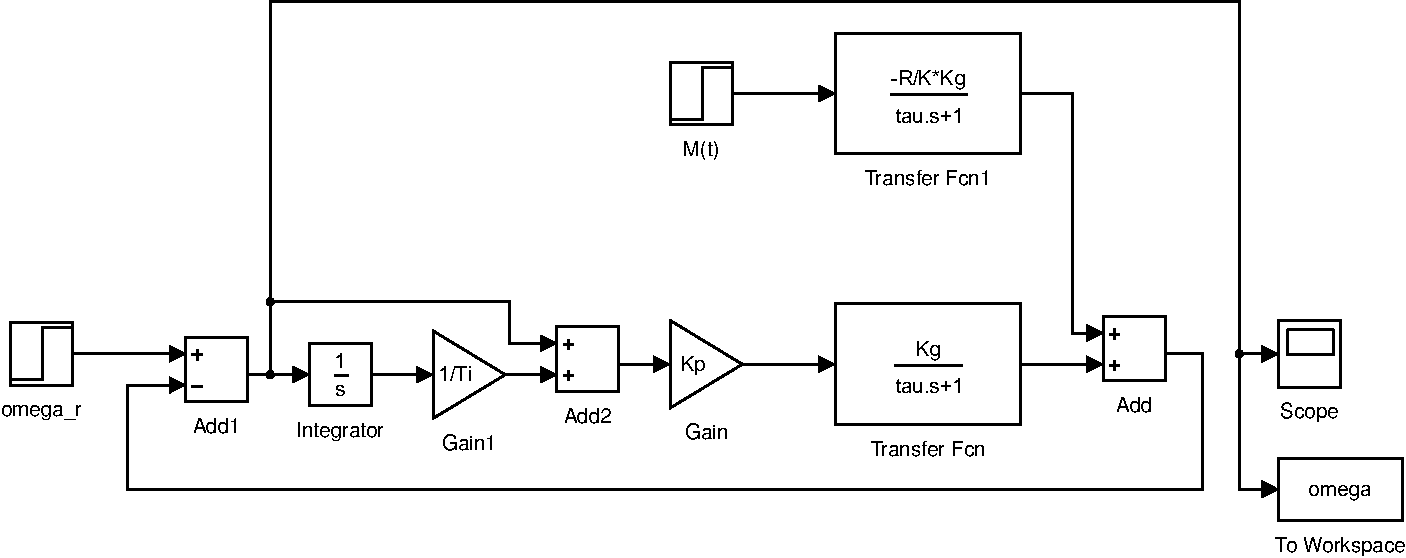
\includegraphics[width=0.6\textwidth]{23/regler_pi_diff.pdf}
    \caption{Regler in Simulink}
    \label{fig:23}
\end{figure}
\begin{figure}[h!]
    \centering
    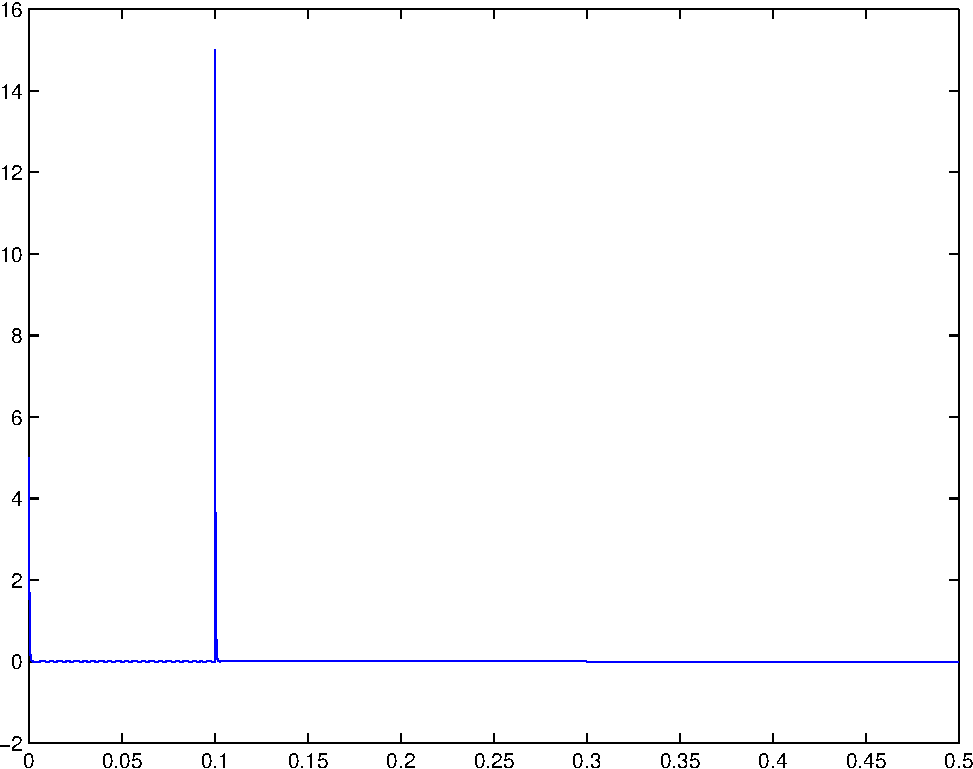
\includegraphics[width=0.6\textwidth]{23/regler_pi_diff_plot.pdf}
    \caption{Simulationsergebnis}
    \label{fig:23plot}
\end{figure}
